%!TEX root=../protocol.tex	% Optional

\section{Zadání}
\subsection{Úvod}
Úloha se věnuje měření optických vláken, jejich vlastností a rušivých jevů souvisejících s vzájemným nedokonalým navázáním v konektorech. Je demonstrován i vliv mechanického namáhání optického vlákna ohyby na malém poloměru křivosti, který se projevuje růstem útlumu. Pro měření se využívá dvou laboratorních elektronických bloků. Blok Tx je vysílací a obsahuje generátory signálu a zdroje záření s LED, IRED (infračerveně emitující dioda), případně laserovou diodou. Blok Rx je přijímací a obsahuje fotodiody, zesilovače a další vyhodnocovací a měřicí obvody.

\subsection{Postup měření}
V rámci měření postupně prověříte vliv různých nedokonalostí v zapojení optických vláken na jejich vlastnosti. Nakonec ověříte vlastnosti WDM přenosu.

\subsection{Závislost útlumu na podélném vychýlení optických kabelů}
Při měření se vyhodnocuje pokles optického výkonu přenášeného mezi vlákny při jejich vzdálení ve směru osy dle obr. 1.
\begin{figure}[h]
\centering
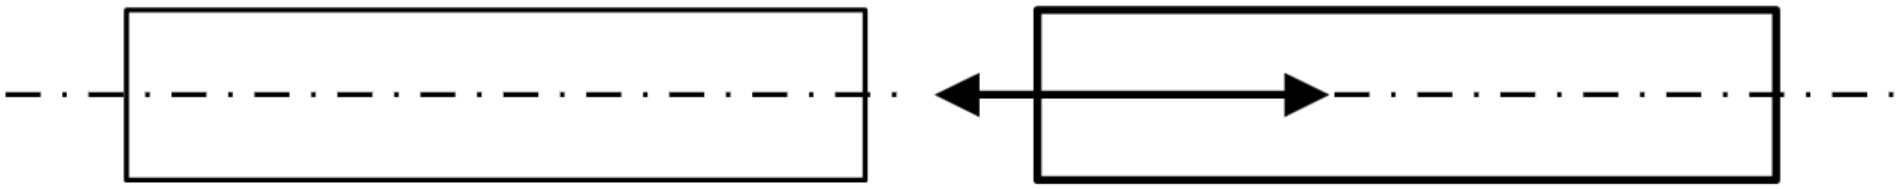
\includegraphics[width=12cm]{images/obr1.png}
\caption{Měření útlumu s podélným posunem vláken}
\label{fig:1}
\end{figure}
\\\\
K měření je využito následujícího zapojení.
\begin{figure}[h]
\centering
\includegraphics[width=12cm]{images/obr2.png}
\caption{Blokové schéma zapojení pro měření útlumu při podélném vychýlení}
\label{fig:2}
\end{figure}
\\\\
Jako optický vysílač použijte LED diodu č. 3 (počítáno shora) na modulu Tx, vlnová délka $\lambda_{max}=660$ nm (červená barva). Jako optický přijímač použijte PIN fotodiodu č. 4 (počítáno shora) na modulu Rx. Na propojení s polohovacím zařízením použijte optické kabely délky 1 m.
\\\\
Nastavte vysílač následovně.

\begin{itemize}
    \item Tlačítkem \textbf{\textit{INPUTS CH.1}} na modulu Tx vyberte jako vstupní zdroj pro kanál 1 vnitřní generátor GEN (indikuje příslušná rozsvícená červená LED dioda v sekci \textbf{\textit{INPUTS}}).
    \item Tlačítkem \textbf{\textit{OUTPUTS CH.1}} na modulu Tx vyberte připojení výstupu kanálu 1 na optický vysílač č. 3 (počítáno shora) - indikuje příslušná rozsvícená červená LED Dioda v sekci \textbf{\textit{OUTPUT SWITCHES}} modulu Tx.
    \item V sekci \textbf{\textit{LF GENERATOR}} modulu Tx vyberte pomocí tlačítka \textbf{\textit{SHAPE}} sinusový tvar průběhu (indikuje příslušná rozsvícená zelená LED dioda) a stisknutím tlačítka \textbf{\textit{1 kHz}} dojde k nastavení frekvence generovaného harmonického signálu na hodnotu 1 kHz.
    \item Pomocí potenciometru \textbf{\textit{P1}} (viz Obr. 2), nacházejícího se v sekci \textbf{\textit{Channel 1}} modulu Tx pod jménem \textbf{\textit{GAIN}}, nastavte maximální zesílení.
    \item Pomocí potenciometru \textbf{\textit{P2}} (viz Obr. 2), nacházejícího se v sekci \textbf{\textit{Channel 1}} modulu Tx pod jménem \textbf{\textit{I-bias}}, nastavte takovou stejnosměrnou složku, aby nedocházelo ke zkreslení harmonického signálu (proudu protékaného LED diodou) – kontrolujte pomocí osciloskopu (viz Obr. 2).
\end{itemize}
\\\\
Nastavte přijímač následovně.
\begin{itemize}
\item Tlačítkem \textbf{\textit{ANALOG IN}} na modulu Rx vyberte jako optický přijímač fotodiodu č. 4 \textbf{\textit{(INPUT 4)}} –indikuje příslušná rozsvícená červená LED dioda v sekci \textbf{\textit{ANALOG}}.
\item Tlačítkem \textbf{\textit{FUNCTION OF OPTICAL POWER METER}} zvolte režim měřiče optického výkonu 1 kHz, což indikuje příslušná rozsvícená červená LED dioda v sekci \textbf{\textit{OPTICAL POWER METER}}.
\item V sekci \textbf{\textit{OPTICAL POWER METER}} vyberte tlačítkem \textbf{\textit{Wavelength}} vlnovou délku na které bude měřen výkon záření. Zvolte hodnotu 660 nm.
\end{itemize}
\\\\
Tímto výše uvedeným nastavením přijímače a vysílače docílíte konfigurace naznačené na Obr. 2.
\\\\
Měření podélného vychýlení proveďte pro rozsah oddálení konektorů x = 0–35 mm (do 10 mm s krokem 1 mm, dále po krocích 5 mm). Pro danou vzdálenost x (viz Obr. 2) odečítejte z displeje přijímače optický výkon jak jednotkách dBm (decibel nad miliwattem), tak v jednotkách W. Přepínání mezi zobrazením optického výkonu v dBm a v $\mu$W se provádí tlačítkem \textbf{\textit{LOG/LIN(dBm/W)}} na modulu Rx. Ověřte platnost převodního vztahu mezi výkonem v jednotkách dBm a výkonem v jednotkách $\mu$W. Vyneste závislost útlumu v jednotkách dB na oddálení konektorů (jako vztažnou hodnotu zvolte výkon změřený při x = 0).

\subsection{Závislost útlumu na úhlovém vychýlení optických konektorů}
Při měření útlumu podle uhlového natočení konců vláken je jedno vlákno pevné a druhé se natáčí v přípravku dle Obr. 3. Při natočení se do přijímacího vlákna postupně dostává menší optický výkon. Při dosažení jistého mezního úhlu do něj již prakticky nevstupuje žádný zářivý tok, i když na vstup vlákna záření stále dopadá.
\begin{figure}[h]
\centering
\includegraphics[width=12cm]{images/obr3.png}
\caption{Měření útlumu s úhlovým natočením konců vláken}
\label{fig:3}
\end{figure}
\\\\
K měření je využitu následující zapojení.
\begin{figure}[h]
\centering
\includegraphics[width=12cm]{images/obr4.png}
\caption{Blokové schéma zapojení pro měření útlumu při úhlovém vychýlení}
\label{fig:4}
\end{figure}
\\\\
Nastavení přijímače a vysílače ponechte shodné s nastavením v předchozím bodě. Měření proveďte pro čelní vzdálenost vláken 5 mm. Úhel natočení měňte v rozsahu x = -25° až +25° s krokem 5°. Výkon odečítejte v jednotkách $\mu$W z displeje přijímače. Vyneste procentuální závislost výkonu na úhlu natočení.
\newpage
\subsection{Stanovení numerické aparatury}
Z výsledků předchozího měření lze také určit numerickou aperturu optického vlákna.
\begin{figure}[h]
\centering
\includegraphics[width=12cm]{images/obr5.png}
\caption{Numerická apertura vlákna}
\label{fig:5}
\end{figure}
\\\\
Numerická apertura je vyjádřena sinem úhlu $\alpha_{mez}$, což je maximální velikost úhlu, který může svírat paprsek s osou optického vlákna, aby při dopadu na jeho čelní plochu byl navázán do vlákna a pokračoval jím. Při praktickém měření se NA určí z úhlu natočení vláken, kdy je pokles přeneseného výkonu na 5 \% původní hodnoty. Pro numerickou aperturu NA optického vlákna platí vztah $NA = \sqrt{n_1^2 - n_2^2}$, kde $n_2$ je index lomu jádra a $n_1$ je index lomu pláště.
\\\\
Z výsledků předchozího měření stanovte numerickou aperturu vlákna. Jako hraniční hodnotu volte 5 \% výkonu v ose vlákna. Porovnejte změřenou NA s hodnotou vypočtenou dle teoretického vztahu, víte-li, že index lomu jádra je 1,49 a pláště 1,41.

\subsection{Závislost útlumu na příčném vychýlení optických konektorů}
Měření při příčném posuvu vláken odpovídá Obr. 6, kdy při rostoucí vzdálenosti roste vložný útlum.
\begin{figure}[ht]
\centering
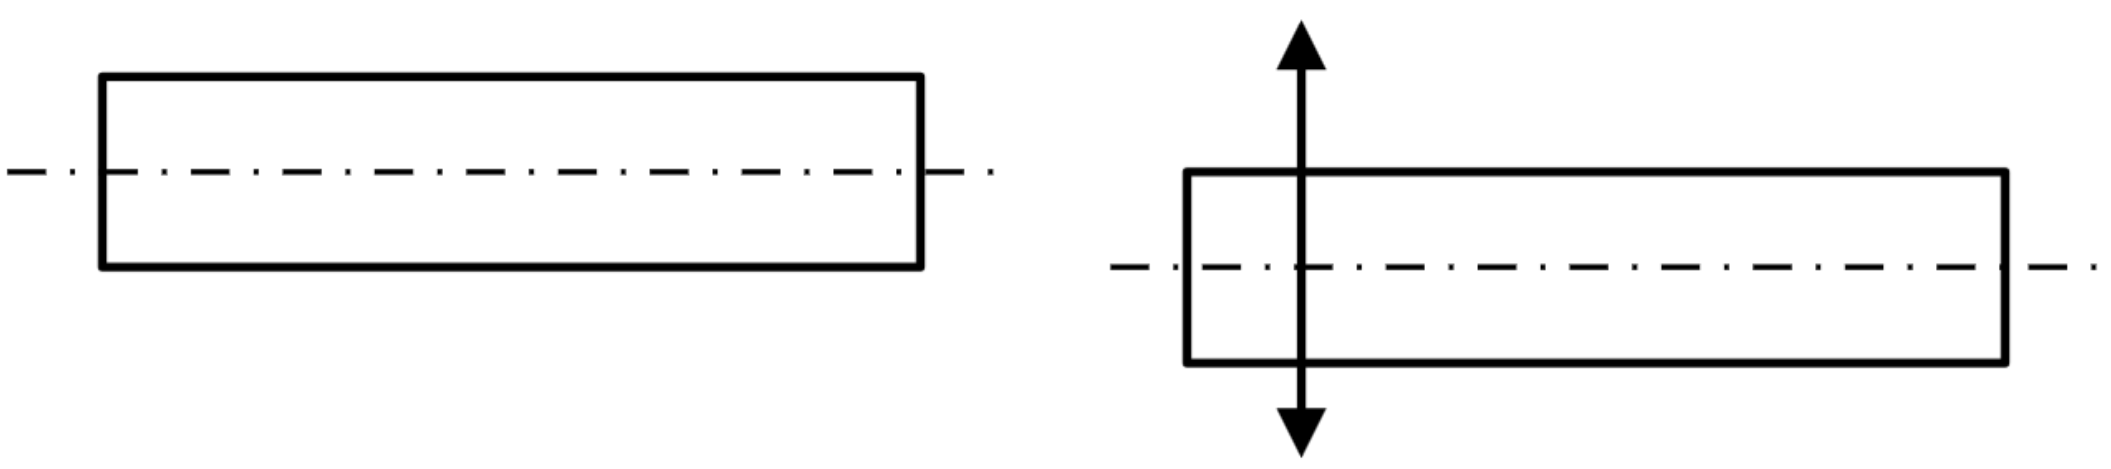
\includegraphics[width=12cm]{images/obr6.png}
\caption{Měření útlumu s příčným posunem vlákna}
\label{fig:6}
\end{figure}
\\\\
K měření je využitu následující zapojení.
\begin{figure}[ht]
\centering
\includegraphics[width=12cm]{images/obr7.png}
\caption{Blokové schéma zapojení pro měření útlumu při příčném vychýlení}
\label{fig:7}
\end{figure}
\\\\
Nastavení přijímače a vysílače ponechte shodné s nastavením v předchozím bodě. Měření proveďte pro rozsah příčného vychýlení konektorů x = -5 až +5 mm s krokem 0,5 mm. Pro danou vzdálenost x odečítejte z displeje přijímače optický výkon v jednotkách dBm. Výkony přepočítejte na útlumy v dB (jako vztažnou hodnotu volte výkon při x = 0). Závislost změřte pro dvě čelní vzdálenosti vláken L = 5 mm a 10 mm. Obě závislosti vyneste do společného grafu.

\subsection{Využití střídavého optického signálu}
Zdůvodněte, proč se v předchozích měřeních používal střídavý optický signál a nikoliv stejnosměrný.

\subsection{Závislost útlumu na ohnutí optického vlákna}
Dalším rušivým působením je namáhání optického vlákna ohybem, při kterém již nemusí být splněny podmínky vedení záření optickým vláknem (z důvodu dopadu paprsku na rozhraní pod úhlem menším - měřeno od kolmice, než je mezní) a záření pak vystupuje z jádra ven.
\begin{figure}[h]
\centering
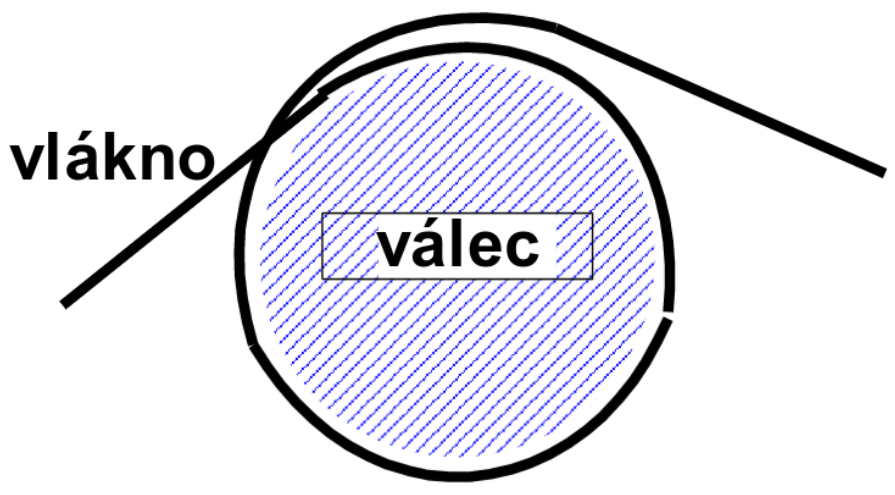
\includegraphics[width=12cm]{images/obr8.png}
\caption{Deformace vlákna při navíjení na válec}
\label{fig:8}
\end{figure}
\\\\
Při měření se tento jev demonstruje optickým vláknem, které se navíjí na válce o různých poloměrech. Při použití stále menšího poloměru válce bude docházet k většímu útlumu. Při použití válce s malým průměrem a červeného světla ve vlákně bude zřetelný jeho únik z pláště.
\\\\
K měření je využito následující zapojení.
\begin{figure}[h]
\centering
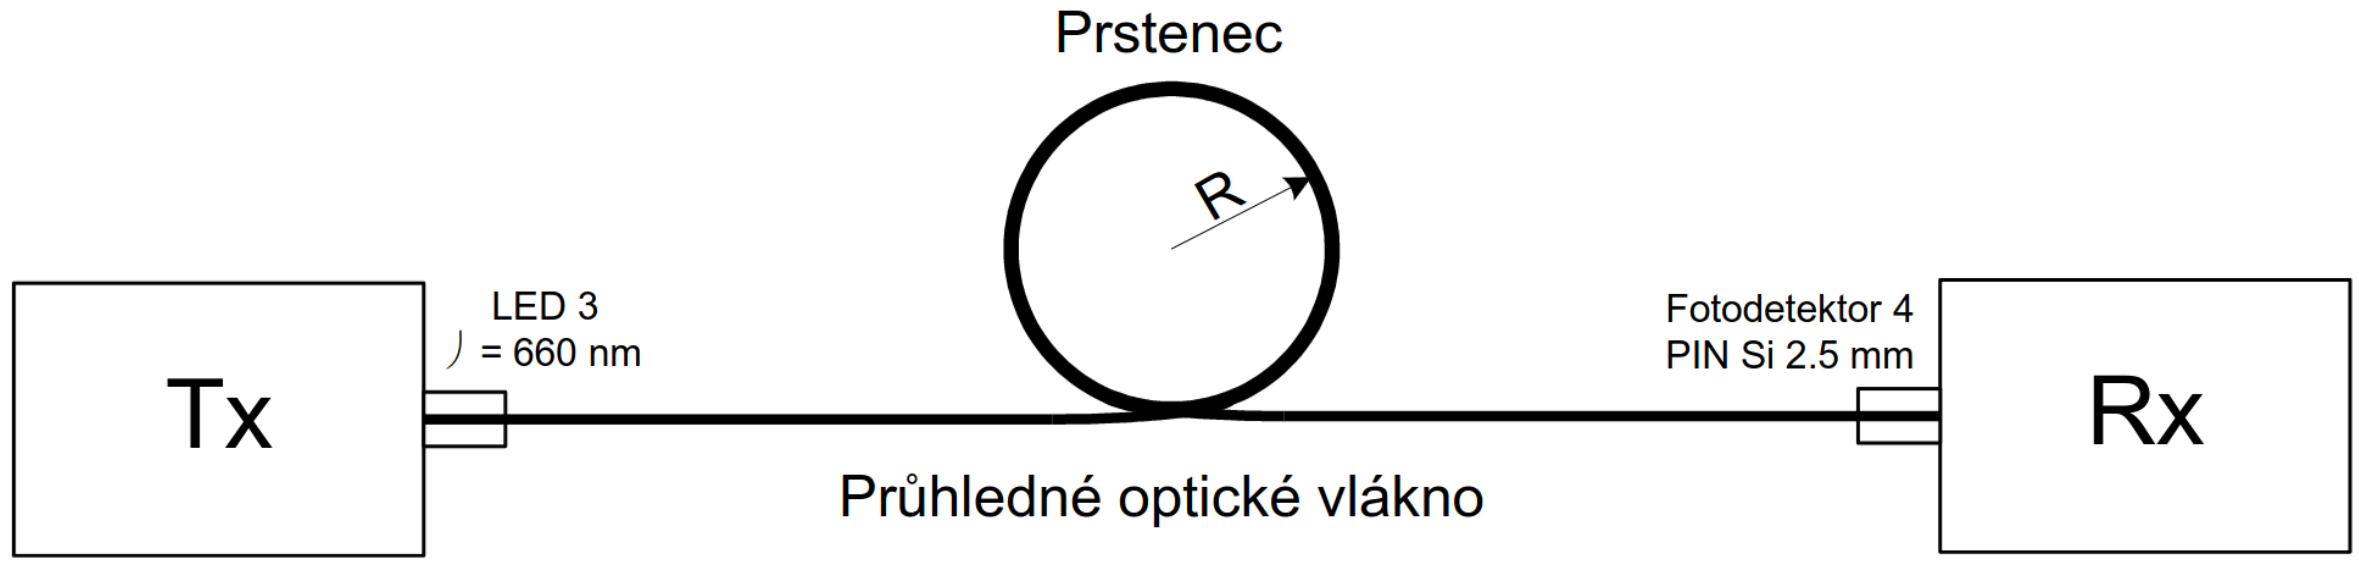
\includegraphics[width=12cm]{images/obr9.png}
\caption{Blokové schéma zapojení pro měření útlumu při ohnutí vlákna}
\label{fig:9}
\end{figure}
\\\\
Nastavení přijímače a vysílače můžete ponechat shodné s nastavením v předchozím bodě. Vysílač s přijímačem spojte pomocí průhledného vlákna. Vlákno opatrně oviňte jednou dokola kolem prstence a ze změny výkonu určete přídavný útlum pro tento ohyb. Měření proveďte pro všechny přiložené prstence o poloměrech R = 1,5 cm, 2,0 cm a 2,5 cm.

\subsection{Spektrální závislost útlumu optických vláken}
K měření je využito následující zapojení.
\begin{figure}[h]
\centering
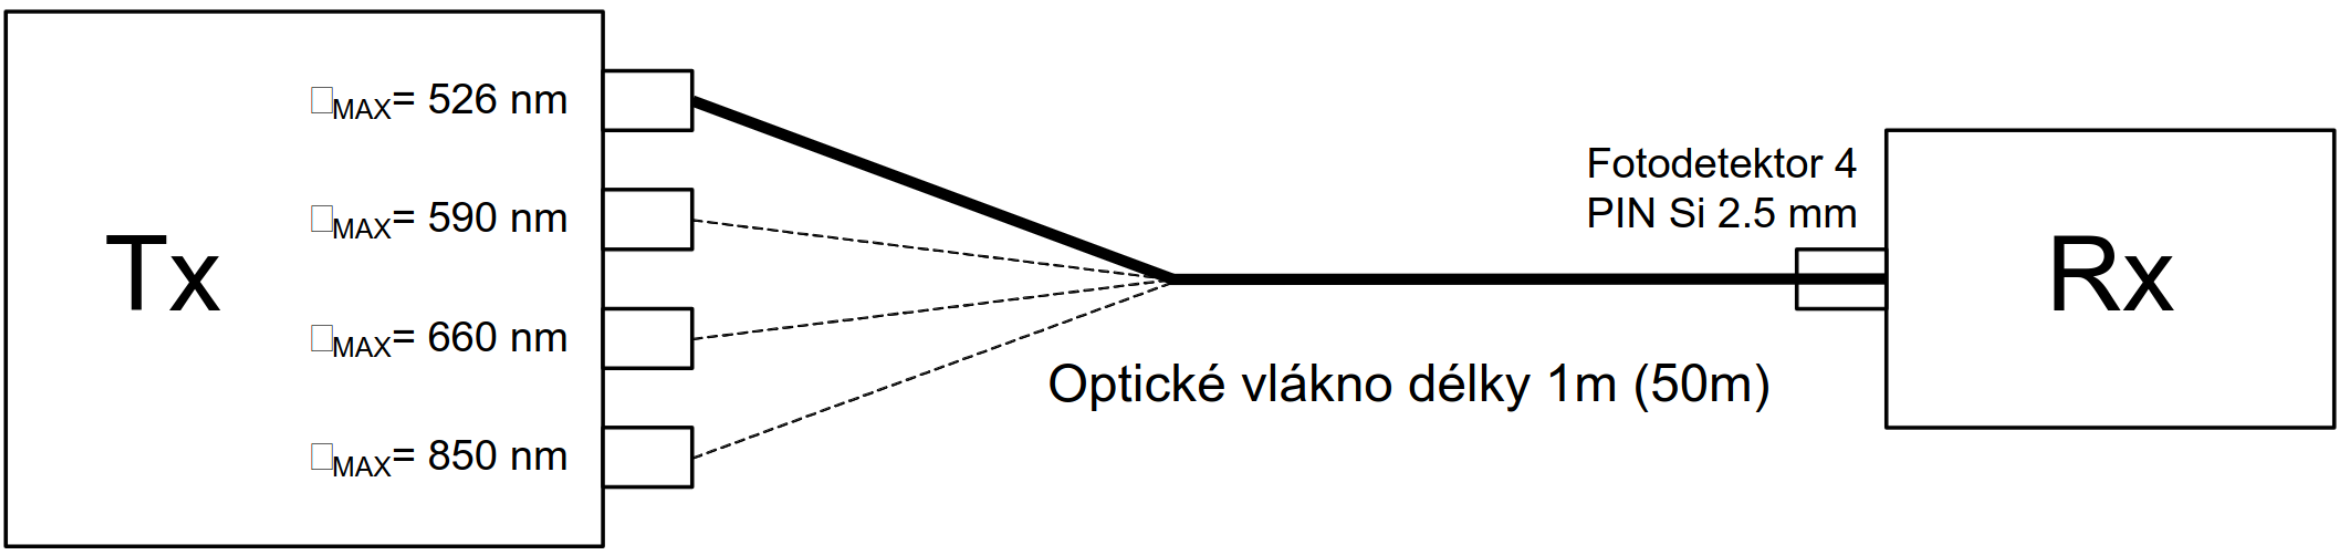
\includegraphics[width=12cm]{images/obr10.png}
\caption{Blokové schéma zapojení pro měření spektrální závislosti útlumu vlákna}
\label{fig:10}
\end{figure}
\\\\
Nastavení přijímače a vysílače můžete nechat shodné s nastavením v bodě 1. Propojte přijímač s vysílačem optickým kabelem délky 1 m. Postupně odečtěte na přijímači výkony v dBm pro první čtyři LED diody vysílače (526 nm, 590 nm, 660 nm a 850 nm). Výstup kanálu vysílače přivedete na příslušnou LED diodu přepínáním pomocí tlačítka \textbf{\textit{OUTPUTS CH1}} na modulu Tx. Stejný postup proveďte též pro optický kabel délky 50 m. Dopočítejte útlumy pro jednotlivé vlnové délky v jednotkách dB/km.
\\\\
Pokud u vlnové délky 850 nm již nebudete schopni na výstupu 50 m optického vlákna výkon změřit (vzhledem k vysokému útlumu), je třeba místo vlákna délky 50 m použít vlákno délky 2 m, které získáte spojením dvou 1 m vláken pomocí ST/ST spojky.

\subsection{Barevný posun světla}
Nastavte jeden konec vlákna dlouhého 50 m proti zdroji bílého světla (např. slunce) a pozorujte barvu na druhém konci vlákna. Na základě výsledků předchozího měření vysvětlete, k čemu došlo.

\subsection{WDM přenos}
Realizujte přenos harmonického signálu z generátoru a řečového signálu z mikrofonu paralelně po jednom optickém vlákně pomocí vlnového multiplexu WDM (Wavelength Division Multiplexing) dle Obr. 11.
\begin{figure}[h]
\centering
\includegraphics[width=12cm]{images/obr11.png}
\caption{Blokové schéma zapojení pro demonstraci WDM a měření přeslechů mezi kanály}
\label{fig:11}
\end{figure}
\\\\
K přenosu použijte dvě LED diody o vlnových délkách 660 nm (LED č. 3) a 850 nm (LED č. 4). Na přijímači vyměňte ST adaptéry bez filtrů na fotodetektorech za ST adaptéry s optickými filtry. Filtr 650 nm našroubujte na fotodetektor 1 a filtr 850 nm na fotodetektor 4 (tím docílíte oddělení signálu na těchto vlnových délkách na vstupu přijímače).
\\\\
Nastavte vysílač následovně.
\begin{itemize}
\item Tlačítkem \textbf{\textit{INPUTS CH.1}} na modulu Tx vyberte jako vstupní zdroj pro kanál 1 vnitřní generátor GEN (indikuje příslušná rozsvícená červená LED dioda v sekci \textbf{\textit{INPUTS}}).
\item Tlačítkem \textbf{\textit{INPUTS CH.2}} na modulu Tx vyberte jako vstupní zdroj pro kanál 2 mikrofon (indikuje příslušná rozsvícená žlutá LED dioda v sekci \textbf{\textit{INPUTS}}).
\item Tlačítkem \textbf{\textit{OUTPUTS CH.1}} na modulu Tx vyberte připojení výstupu kanálu 1 na optický vysílač č. 3 (počítáno shora) - indikuje příslušná rozsvícená červená LED dioda v sekci \textbf{\textit{OUTPUT SWITCHES}} modulu Tx.
\item Tlačítkem \textbf{\textit{OUTPUTS CH.2}} na modulu Tx vyberte připojení výstupu kanálu 2 na optický vysílač č. 4 (počítáno shora) - indikuje příslušná rozsvícená žlutá LED dioda v sekci \textbf{\textit{OUTPUT SWITCHES}} modulu Tx.
\item V sekci \textbf{\textit{LF GENERATOR}} modulu Tx vyberte pomocí tlačítka \textbf{\textit{SHAPE}} harmonický průběh (indikuje příslušná rozsvícená zelená LED dioda) a stisknutím tlačítka \textbf{\textit{1 kHz}} dojde k nastavení frekvence generovaného harmonického signálu na hodnotu 1 kHz.
\item Pomocí potenciometru \textbf{\textit{P1}} (viz Obr. 11), nacházejícím se v sekci \textbf{\textit{Channel 1}} modulu Tx pod jménem \textbf{\textit{GAIN}}, nastavte maximální zesílení kanálu 1.
\item Pomocí potenciometru \textbf{\textit{P2}} (viz Obr. 11), nacházejícím se v sekci \textbf{\textit{Channel 1}} modulu Tx pod jménem \textbf{\textit{I-bias}}, nastavte takovou stejnosměrnou složku, aby nedocházelo ke zkreslení sinusového signálu (sinusového proudu protékaného LED diodou) – kontrolujte pomocí osciloskopu (viz Obr. 11).
\item Pomocí potenciometru P3 a P4 (viz Obr. 11), nacházející se v sekci \textbf{\textit{Channel 2}} modulu Tx pod jménem \textbf{\textit{GAIN}} a \textbf{\textit{I-bias}}, nastavte takové zesílení a takovou stejnosměrnou složku, aby nedocházelo k přebuzení kanálu a zkreslení přenášeného signálu z mikrofonu (proudu protékaného LED diodou) - kontrolujte pomocí osciloskopu.
\end{itemize}
\\\\
Přijímač nastavte následovně.
\begin{itemize}
\item Potenciometrem \textbf{\textit{P1 (GAIN)}} je možno řídit zisk kanálu a potenciometrem \textbf{\textit{P3 (Volume)}} hlasitost reproduktoru.
\item Potenciometr \textbf{\textit{P2}} (stejnosměrný posun signálu na výstupu) stáhněte na minimum (nulový stejnosměrný posun).
\item Tlačítkem \textbf{\textit{ANALOG IN}} na modulu Rx je možno se přepínat mezi optickým přijímačem fotodioda č.1 \textbf{\textit{(INPUT 1)}} a fotodioda č.4 – indikuje příslušná rozsvícená červená LED dioda v sekci \textbf{\textit{ANALOG}}.
\end{itemize}
\\\\
Nejprve ověřte přítomnost přeslechu mezi kanály. Sledujte na osciloskopu přeslech harmonického signálu z kanálu 1 do řečového signálu v kanálu 2 a opačně. Sledujte tyto přeslechy též poslechem reproduktoru.
\\\\
Poté proveďte měření přeslechu mezi kanály. Pomocí potenciometru \textbf{\textit{P3}} nastavte zesílení kanálu 2 (řečový signál) na minimum. Změřte amplitudu harmonického signálu na výstupu přijímače v kanále vlnové délky 660 nm (fotodioda 1) a amplitudu harmonického signálu přenášeného přeslechem do kanálu vlnové délky 850 nm (fotodioda 4). Vypočítejte úroveň přeslechu z kanálu 660 nm do kanálu 850 nm v dB. Pomocí tlačítek \textbf{\textit{OUTPUTS CH.1}} a \textbf{\textit{OUTPUTS CH.2}} na modulu Tx vzájemně přehoďte výstupy na LED diody (tzn. po 660 nm se bude přenášet řečový signál a po 850 nm harmonický signál z generátoru) a změřte přeslech kanálu 850 nm do kanálu 660 nm.
\\\\
Po ukončení měření vyměňte ST adaptéry s optickými filtry na fotodetektorech za ST adaptéry bez filtrů.
\textbf{\textit{}}